\documentclass[12pt,a4paper]{ouparticle}
% \documentclass{article}
% \usepackage[T1]{fontenc}
\usepackage{mathptmx}
\usepackage{times}
\usepackage[flushleft]{threeparttable}
\usepackage{graphicx}
\setlength\parindent{12pt} 

\usepackage{natbib}
\usepackage{rotating} % Load the rotating package
\usepackage[hidelinks]{hyperref}
\hypersetup{
  colorlinks   = true, %Colours links instead of ugly boxes
  urlcolor     = blue, %Colour for external hyperlinks
  linkcolor    = blue, %Colour of internal links
  citecolor   =  red %Colour of citations
}
\usepackage{xcolor}

\newtheorem{hyp}{Hypothesis}
\makeatletter
\newcounter{subhyp} 
\let\savedc@hyp\c@hyp
\newenvironment{subhyp}
 {%
  \setcounter{subhyp}{0}%
  \stepcounter{hyp}%
  \edef\saved@hyp{\thehyp}% Save the current value of hyp
  \let\c@hyp\c@subhyp     % Now hyp is subhyp
  \renewcommand{\thehyp}{\saved@hyp\alph{hyp}}%
 }
 {}
\newcommand{\normhyp}{%
  \let\c@hyp\savedc@hyp % revert to the old one
  \renewcommand\thehyp{\arabic{hyp}}%
} 

\doublespacing

\begin{document}

%\title{Referee Report}
\title{%
  Macroeconomic factor models   \\
  \large Report}

\author{%
\name{Xuanheng Huang}}

\date{\today}

\maketitle


\section{Introduction}
In this report, I examine the following paper: "Macroeconomic risks and characteristic-based factor models." by Aretz, Kevin, Söhnke M. Bartram, and Peter F. Pope, published in the Journal of Banking \& Finance. In section 2, I show the replication of the main results. In section 3, I highlight the strengths and weaknesses of the paper. In the last part, section 4, I propose some extensions of the paper. 


\section{Replication}
Table 1 shows the estimation results for the mimicking portfolios for industrial production growth. The original paper uses bond returns data from Ibbotson Associates. I do not have access to this database, I use the bond returns data from Bloomberg. Table 2 shows the summary statistics of the macroeconomic variables that are used in the macroeconomic factor model. The changes in the survival probability have public data only until 1999. I extended the data to the period from 2000 to 2008 \footnote{The Pearsons' correlation between the monthly DSV series obtained from Maria Vassalou’s website and mine is $0.712$}. Table 3 shows the Granger causality results between the macroeconomic variables and financial factors (book-to-market ratio, size, and momentum). Figure 1 shows the beta estimates from the GMM of the one-way sorted firm characteristic deciles. 

\begin{table}
  \begin{threeparttable}
    \caption{Estimation of the mimicking portfolio for industrial production growth}
    {
\def\sym#1{\ifmmode^{#1}\else\(^{#1}\)\fi}
\begin{tabular}{@{\extracolsep{2pt}}l*{2}{c}@{}}
\hline\hline


 & Ind. productivity growth & Ind. productivity growth \\
\hline
Market portfolio ex. return ($RM_{t-1,t}$) & 0.130 & 0.131 \\
 & (1.547) & (1.515) \\
10-year gov. bond ex. return$_{t-1,t}$ & -0.348\sym{**} & -0.424\sym{**} \\
 & (-2.509) & (-2.262) \\
5-year gov. bond ex. return$_{t-1,t}$ & 0.316\sym{*} & 0.465\sym{**} \\
 & (1.784) & (2.057) \\
Gold ex. returns$_{t-1,t}$ & -0.039 & -0.048\sym{*} \\
 & (-1.452) & (-1.699) \\
Slope dummy mkt portfolio ex. return (87) & -0.079 & -0.081 \\
 & (-0.865) & (-0.968) \\
Slope dummy mkt portfolio ex. return (96-02) & 0.009 & 0.010 \\
 & (0.084) & (0.094) \\
Intercept & 0.025 & 0.026\sym{*} \\
 & (1.606) & (1.703) \\
Risk-free rate of return & -8.787\sym{**} & -9.457\sym{**} \\
 & (-2.031) & (-2.253) \\
10-year minus 3-month gov. bond yield$_{t-1}$ & -0.039 & -0.114 \\
 & (-0.070) & (-0.210) \\
1-year minus 3-month gov. bond yield$_{t-1}$ & 1.814\sym{**} & 1.650\sym{**} \\
 & (2.459) & (2.282) \\
Baa minus Aaa corporate bond yield$_{t-1}$ & -0.352 & -0.298 \\
 & (-0.215) & (-0.185) \\
Dividend yield$_{t-1}$ & 1.656\sym{***} & 1.796\sym{***} \\
 & (2.938) & (3.184) \\
Industrial production growth$_{t-13,t-1}$ & 0.155 & 0.137 \\
 & (1.311) & (1.275) \\
Inflation$_{t-13,t-1}$ & -0.488\sym{**} & -0.510\sym{**} \\
 & (-2.265) & (-2.255) \\
Market portfolio ex. return ($RM_{t-13,t-1}$) & 0.108\sym{***} & 0.101\sym{***} \\
 & (5.418) & (5.589) \\
1-month lagged base asset returns & No & Yes \\

\hline
Obs & 400 & 400 \\
Adj. R\sym{2} & 0.382 & 0.390 \\
F-stat & 10.252 & 8.595 \\
\hline\hline
\end{tabular}
}
    \begin{tablenotes} 
    \footnotesize
    \item This table shows the outcomes from OLS estimations of the log change in industrial production over the next year onto on a set of base asset excess returns and lagged control variable realizations. The base assets consist of the market portfolio, two government bond portfolios, a default bond portfolio, and gold. To allow for time-variation in the market portfolio weight, the regression includes two market portfolio slope dummies for the period from April 1987 to April 1988 (the one year surrounding the October 1987 stock market crash) and the period from January 1996 to December 2002 (the Internet bubble period). All base asset returns are in excess of the risk-free rate of return, and thus weights do not need to sum up to unity. The regressions control for the expected level of returns by including a set of lagged control variables, containing the risk-free rate, the yield spread between long-term and short-term government bonds, the yield spread between one-year and short-term government bonds, the yield spread between Baa-rated and Aaa-rated corporate bonds and the dividend yield on the S\&P 500. Controls include industrial production growth, inflation and excess market returns over the last year. Since realized industrial production growth has an overlap with its lagged value of eleven months, the variances have the Newey and West (1987) correction with $l = 11$. The sample period extends from January 1978 to April 2008.
    \end{tablenotes}
  \end{threeparttable}
\end{table}

\begin{sidewaystable}
  \begin{threeparttable}
    \caption{Summary statistics}
    \begin{tabular}{lrrrrrrrr} 
 \hline 
 \hline
 & N & Mean ($\times 10^3$) & Std. dev. ($\times 10^3$) & Min. ($\times 10^3$) & 25\% ($\times 10^3$) & Median ($\times 10^3$) & 75\% ($\times 10^3$) & Max. ($\times 10^3$) \\
\hline 
 MYP & 400 & 0.777 & 6.694 & -22.303 & -3.196 & 1.020 & 4.870 & 22.770 \\
UI & 400 & -0.082 & 2.833 & -11.771 & -1.781 & -0.126 & 1.546 & 9.222 \\
DSV & 400 & 0.348 & 6.895 & -35.000 & -2.254 & 0.300 & 3.000 & 52.100 \\
ATS & 400 & -0.116 & 4.040 & -28.650 & -1.500 & -0.100 & 1.750 & 18.000 \\
STS & 400 & 0.050 & 4.272 & -15.100 & -2.200 & -0.300 & 2.000 & 21.300 \\
FX & 400 & -0.764 & 19.001 & -65.885 & -12.221 & -0.323 & 10.655 & 72.889 \\

 \hline \hline 
 \end{tabular}

    \begin{tablenotes} 
    \small 
    \item This table provides summary statistics on the analysis variables. The sample period extends from January 1978 to April 2008.
    \end{tablenotes}
  \end{threeparttable}
\end{sidewaystable}

\begin{table}
\centering
  \begin{threeparttable}
    \caption{VAR estimation}
    \begin{tabular}{l*{9}{c}}
\hline
\hline
& HML& SMB& WML& MYP& UI& DSV& ATS& STS& FX\\
\hline
Constant & 0.00 & 0.00 & 0.01 & 0.00 & -0.00 & -0.00 & -0.00 & 0.00 & -0.00\\
   & (2.19) & (1.35) & (4.15) & (0.37) & (-0.58) & (-0.10) & (-1.02) & (0.55) & (-0.31)\\
HML & 0.22 & -0.03 & -0.10 & -0.01 & 0.00 & 0.00 & 0.01 & -0.01 & -0.01\\
   & (3.60) & (-0.49) & (-1.16) & (-0.77) & (0.64) & (0.18) & (0.78) & (-0.70) & (-0.25)\\
SMB & 0.12 & -0.05 & 0.12 & 0.02 & 0.01 & 0.03 & 0.01 & -0.00 & -0.01\\
   & (2.13) & (-0.80) & (1.40) & (1.32) & (1.84) & (2.61) & (0.95) & (-0.60) & (-0.35)\\
WML & -0.09 & -0.10 & -0.05 & -0.00 & 0.01 & -0.01 & 0.00 & -0.01 & -0.03\\
   & (-2.42) & (-2.36) & (-0.82) & (-0.60) & (1.73) & (-1.41) & (0.79) & (-1.15) & (-1.23)\\
MYP & 0.48 & 1.01 & -1.00 & 0.13 & 0.05 & 0.11 & 0.15 & -0.10 & 0.08\\
   & (1.26) & (2.39) & (-1.76) & (1.52) & (1.40) & (1.45) & (2.86) & (-1.83) & (0.31)\\
UI & 0.59 & -1.09 & -0.09 & -0.01 & 0.37 & -0.13 & 0.08 & 0.12 & -0.04\\
   & (1.10) & (-1.82) & (-0.12) & (-0.05) & (7.38) & (-1.19) & (1.09) & (1.46) & (-0.11)\\
DSV & 0.05 & 0.05 & 0.28 & 0.09 & -0.04 & 0.24 & 0.05 & -0.01 & 0.38\\
   & (0.16) & (0.14) & (0.60) & (1.31) & (-1.41) & (3.87) & (1.08) & (-0.22) & (1.78)\\
ATS & -1.13 & -1.32 & 1.49 & -0.05 & 0.02 & -0.42 & 0.10 & -0.11 & 0.60\\
   & (-2.10) & (-2.21) & (1.85) & (-0.43) & (0.48) & (-3.98) & (1.29) & (-1.41) & (1.65)\\
STS & -0.71 & -0.09 & 0.09 & 0.02 & 0.01 & -0.07 & 0.00 & 0.08 & 0.42\\
   & (-1.79) & (-0.21) & (0.14) & (0.24) & (0.25) & (-0.85) & (0.00) & (1.29) & (1.56)\\
FX & 0.15 & 0.01 & 0.00 & -0.04 & -0.00 & -0.01 & -0.03 & 0.03 & 0.13\\
   & (1.96) & (0.11) & (0.00) & (-2.08) & (-0.54) & (-0.77) & (-2.82) & (2.51) & (2.40)\\
\hline
\hline
\end{tabular}

    \begin{tablenotes} 
    \small 
    \item This table reports the empirical outcomes from estimations of VAR systems on the Fama and French and Carhart benchmark factors, i.e., HML, SMB and WML, and the macroeconomic fundamentals. The macroeconomic fundamentals are the mimicking portfolio on changes in industrial production growth expectations (MYP), unexpected inflation (UI), changes in the survival probability (DSV), changes in the average level of the term structure of risk-free interest rate yields (ATS), changes in the slope of the term structure of risk-free interest rate yields (STS) and changes in the exchange rate between the US dollar and a trade-weighted composite currency (FX). This table uses monthly data from January 1978 to April 2008 with a lag size equal to one. Numbers in parentheses are t-statistics.
    The independent variables are lagged by one period.
    \end{tablenotes}
  \end{threeparttable}
\end{table}


\begin{figure}
\centering
    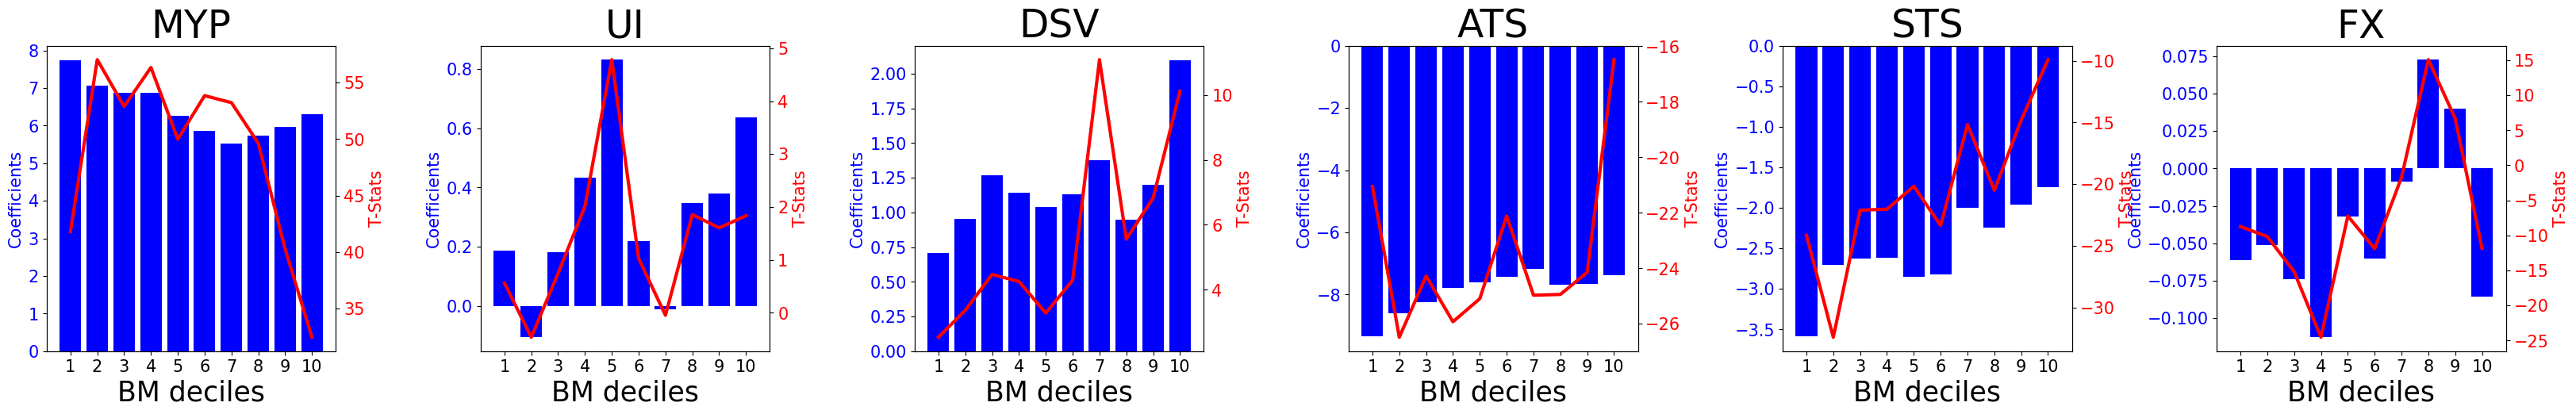
\includegraphics[width=16cm]{plots/betahist1.png}\\
    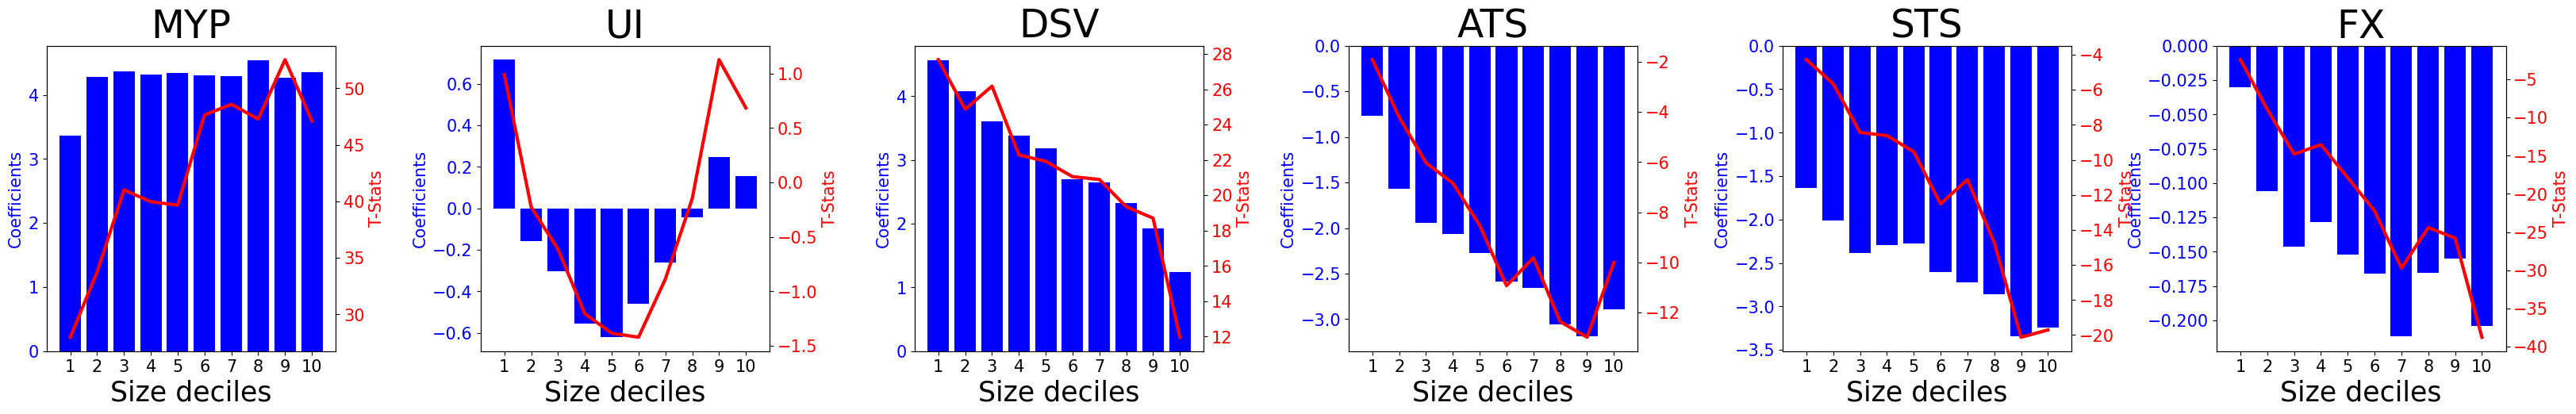
\includegraphics[width=16cm]{plots/betahist2.png}\\
    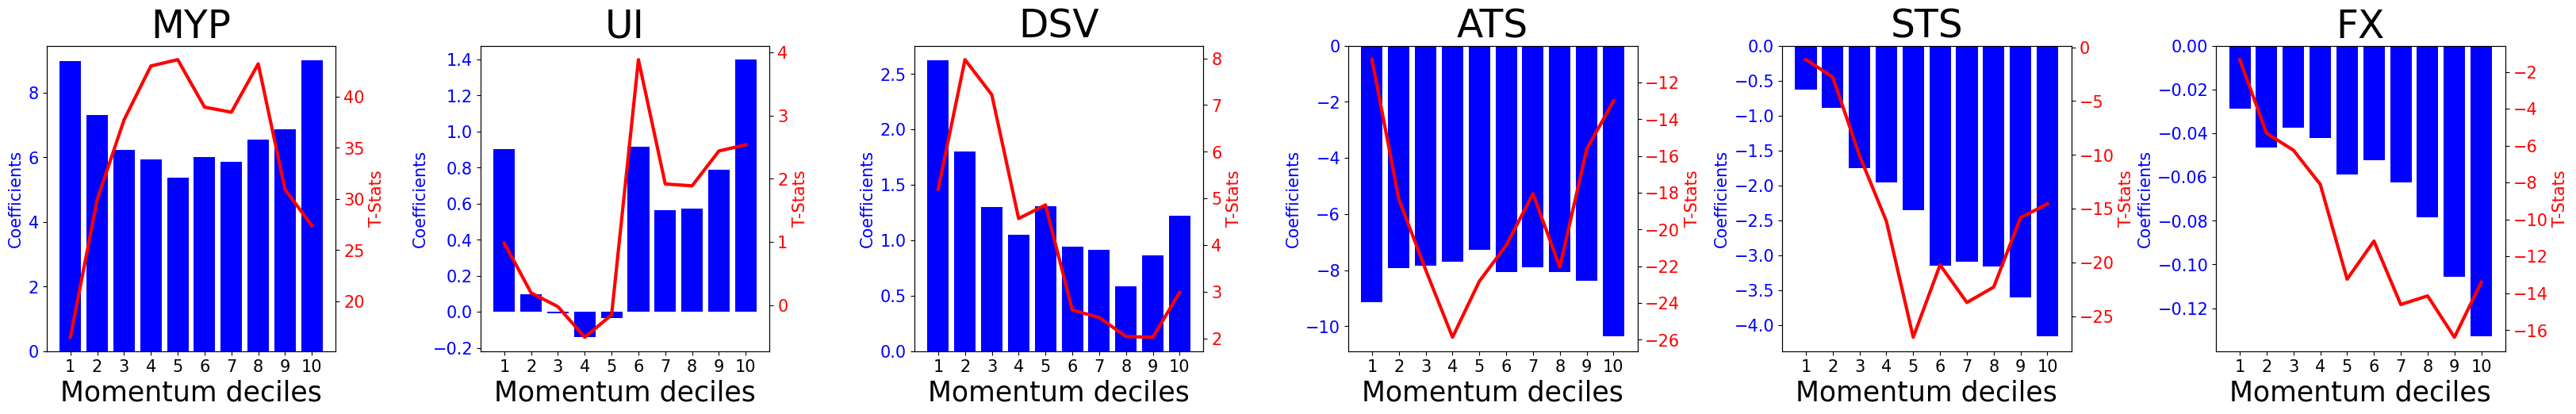
\includegraphics[width=16cm]{plots/betahist3.png}
% \captionsetup{labelformat=empty}
  \caption{This figure shows the macroeconomic risk exposure estimates of the one-way sorted firm characteristic deciles on the macroeconomic fundamentals and their statistics. The macroeconomic fundamentals are changes in industrial production growth expectations (MYP), unexpected inflation (UI), changes in the aggregate survival probability (DSV), changes in the average level and the slope of the term structure of risk-free interest rate yields (ATS and STS, respectively), and changes in the exchange rate between the US dollar and a trade-weighted composite currency (FX). The blue bars are the estimated risk exposures, while the red lines are the t-statistics. The first row shows the outcomes related to the one-way sorted book-to-market deciles, the second those related to the one-way sorted size deciles, and the third those related to the one-way sorted momentum deciles.}
\end{figure}

% \begin{table}
%   \begin{threeparttable}
%     \caption{Estimation of Risk premia}
%     \begin{tabular}{l*{1}{c}}
\hline
\hline
& Market price of risk ($\lambda$) (\times 100)\\
\hline
MYP & -1.39\\
   & (-0.08)\\
UI & 11.82\\
   & (0.01)\\
DSV & -8.54\\
   & (-0.01)\\
ATS & -21.56\\
   & (-0.01)\\
STS & 17.77\\
   & (0.01)\\
FX & -134.65\\
   & (-0.00)\\
\hline
\hline
\end{tabular}

%     % \begin{tabular}{l*{1}{c}}
\hline
\hline
& Market price of risk ($\lambda$) (\times 100)\\
\hline
MYP & -0.18\\
   & (-779.56)\\
UI & -0.04\\
   & (-249.39)\\
DSV & 0.30\\
   & (2384.42)\\
ATS & -0.20\\
   & (-720.55)\\
STS & -0.04\\
   & (-172.85)\\
FX & -1.22\\
   & (-128.27)\\
\hline
\hline
\end{tabular}

%     % \begin{tabular}{l*{1}{c}}
\hline
\hline
& Market price of risk ($\lambda$) (\times 100)\\
\hline
MYP & -1.10\\
   & (-3.02)\\
UI & 0.81\\
   & (3.49)\\
DSV & -1.11\\
   & (-8.05)\\
ATS & -1.30\\
   & (-3.20)\\
STS & 1.46\\
   & (2.63)\\
FX & -29.40\\
   & (-0.18)\\
\hline
\hline
\end{tabular}

%     \begin{tablenotes} 
%     \footnotesize
%     \item asdfa
%     \end{tablenotes}
%   \end{threeparttable}
% \end{table}


\section{Referee's report}
Prior research has demonstrated how various macroeconomic factors can account for financial market returns. However, these studies appear to be disconnected from one another, posing a problem as many of these macroeconomic fundamentals are interrelated and likely overlap in their explanations. This study provides a comprehensive analysis that explores the connections between multiple macroeconomic factors, and proposes a model based on these findings. Additionally, the results reveal that the macroeconomic fundamentals model provides similar results to the 3-factor Fama-French model and can partially account for the momentum factor. This finding is significant because the 3-factor model plus momentum lacks a theoretical basis, while results suggest that the financial factors may be reflecting exposure to macro factors.

In terms of implementation, the paper faces several challenges. The first factor, $MYP_{t,t+12}$, conceptually captures news related to economic growth and measures the change in economic growth expectations. As GDP growth is only observable on a quarterly basis, the authors use a different proxy, the industrial production index, which is observable monthly. However, unlike GDP, which reflects the general condition of the economy, industrial production is more specific to the total output produced and does not account for the price paid by the final consumer or the value-added in the retail sector. It would be advisable to follow the same approach as \cite{vassalou2003news} and use GDP data for the quarterly-level analyses. Additionally, in the estimation of the mimicking portfolio, the problem of overlap of eleven months can be avoided, as in the original tables realized industrial production growth has eleven months in common with its lagged value.

The authors of the paper construct a mimicking portfolio to capture all anticipated information regarding future economic changes over the next year. Assuming that industrial production growth is an adequate proxy for overall economic growth, there are still three main issues to consider. First, the researcher must decide which financial factors to include in the estimation of the mimicking portfolio. This is a challenging task as it is difficult to include a comprehensive list of assets that incorporates information regarding future economic growth. As a result, there is a risk of omitted variables, which could bias the estimation of the change in economic growth expectation. To address this issue, the authors could employ alternative and more direct measures of changes in economic growth to show the robustness of the results. The paper does show that the factor $MYP_{t,t+12}$ and the Livingston Surveys of Professional Forecasters have a correlation of around 50\%, but it would be interesting to repeat the analysis with alternative measures included as a factor in the proposed factor model.

Secondly, the proposed method only captures the change in expectation of one-year economic growth. However, the literature \citep{bansal2004risks} suggests that changes in long-term economic growth also play a crucial role in explaining high-risk premia observed in financial markets. Therefore, it would be interesting to extend the proposed model to incorporate long-term growth expectations and examine how they affect asset prices.

Thirdly, one of the key assumptions of the proposed model is that investors' perception of news remains constant over time. However, investors may perceive news differently depending on the current level of optimism or pessimism, leading to overreactions or underreactions. The inclusion of dummy variables in the picking portfolio regression, such as the slope dummy for the market portfolio excess return in 1987 and 1999-2002, is likely to be correlated with general market sentiment. The choice of the specific years for the introduction of these dummy variables may seem somewhat arbitrary. An alternative approach could be to use direct measures of market sentiment, such as textual analysis of newspaper headlines, to capture changes in investor perception over time.

As for other proposed macroeconomic variables, one alternative to using the measure of unexpected inflation is to use the Inflation Expectation from the University of Michigan, which is based on Surveys of Consumers. This measure is a direct measure and does not require the estimation used in the original measure. However, it may be subject to measurement error due to the nature of surveys.

In the paper, it is not entirely clear how certain variables are constructed. For instance, the authors do not provide sufficient details on how the long- and medium-term government bond portfolios are formed.

Additionally, regarding the table showing the results of the mimicking portfolio estimation, the authors do not explain much the results. It would be helpful if the authors provided more discussion on their findings, particularly those that contrast with previous studies. For example, \cite{vassalou2003news} found that the return on long-term government bonds minus the return on short-term government bonds has a positive coefficient in explaining future changes in GDP. However, in this paper, the long-term government bond has a positive coefficient in explaining future changes in industrial production.

Overall, while the paper presents numerous correlation results, it lacks a strong theoretical framework to support them. The authors do conduct a Granger causality analysis, but further discussion on their findings would be beneficial. This is particularly true for results that are in contrast with previous findings. Such discussion would be useful in their analysis of the relationship between Fama-French and momentum factors and the macro factor model. It would help us better understand why certain characteristics make firms more or less sensitive to macroeconomic shocks.
 

\section{Proposal (further studies)}
A potential extension of this study would be to expand the sample period to include data from the last decade and repeat the analysis. This would allow us to determine whether the results still hold after the financial crisis. Additionally, such an analysis could provide insights into why the performance of the value premium has weakened.
 
To enhance the performance of the macroeconomic factor model, we could incorporate additional factors that have recently been shown to play a significant role in explaining fluctuations in financial markets. For instance, we could include the level of government debt as a factor. This variable can affect incentives to innovate and, consequently, future prospects \citep{croce2019government}. 

Furthermore, we could enhance the model by incorporating macroeconomic factors that have not been widely used. For instance, we could include the ratio of middle-aged to young populations as a factor. Different age groups tend to have different investment preferences, so this variable could provide valuable insights.

Additionally, we could expand the characteristic-based model to include the Fama-French five-factor model \citep{fama2015five} by incorporating profitability, investment, and momentum factors. It would be particularly interesting to examine how profitability and investment are related to sensitivity to macroeconomic factors. Another model worth exploring is the q-theory factor model \citep{hou2015digesting,hou2021augmented}. We could investigate how each of its factors - profitability, investment, and expected investment growth - are related to macroeconomic factors. This would be a valuable contribution, as the q-theory model is more theory-based. 

% I expect profitability risk to be highly correlated with changes in economic growth prospects. On the other hand, I expect the investment to be related to change in the average s

% I predict profitability to be...
% investment to be ...
% expected investment growth to be..



\newpage

\bibliographystyle{chicago}
\bibliography{bibliography}

\end{document}